\section{Feature Extraction}
\label{feature-extract:sec}

%Tien
%The goal of this step is to extract the important features for FL from
%the test coverage and the given source code and its repository.



\subsection{Method-level Feature Extraction}

Figure~\ref{method-level-feature-extraction} illustrates the key
attributes and relations that we collect for each method $M_1$. We
extract the following \underline{attributes} for
$M_1$.

1) {\em \underline{The method's content}}: we remove special
characters and separators in the method's interface and body, and use
naming convention to break each code token into the sub-tokens. For
example, in Figure~\ref{method-level-feature-extraction}, the node
$M_1$ represents the method \code{computeGeometricalPro\-perties} in
Figure~\ref{statement-level-feature-extraction}. For the content for
$M_1$, the extracted sequence of sub-tokens is \code{protected},
\code{void}, \code{compute}, \code{Geometrical}, \code{Properties},
etc.

2) {\em \underline{The method's structure}}: the corresponding parser
is used to build the AST of the method (e.g., JDT~\cite{JDT} for Java
code).

%we use JDT package~\cite{JDT} to parse the source code to build the
%AST of the method.

3) {\em \underline{Most similar faulty method}}: we keep the most
similar faulty method $M_b$ with $M_1$. Note that we keep $M_b$ as an
attribute of $M_1$, rather than representing $M_b$ in the feature
graph. The rationale is that $M_b$ might be in the past and might not
be present in the current version of the project. Two methods are
similar when they have similar sequences (measured by the cosine
similarity) of the sub-tokens (represented by the GloVe
embeddings~\cite{glove2014}).  For $M_b$, we build its AST and
keep as an attribute for $M_1$.

  \begin{figure}[t]
	\centering
	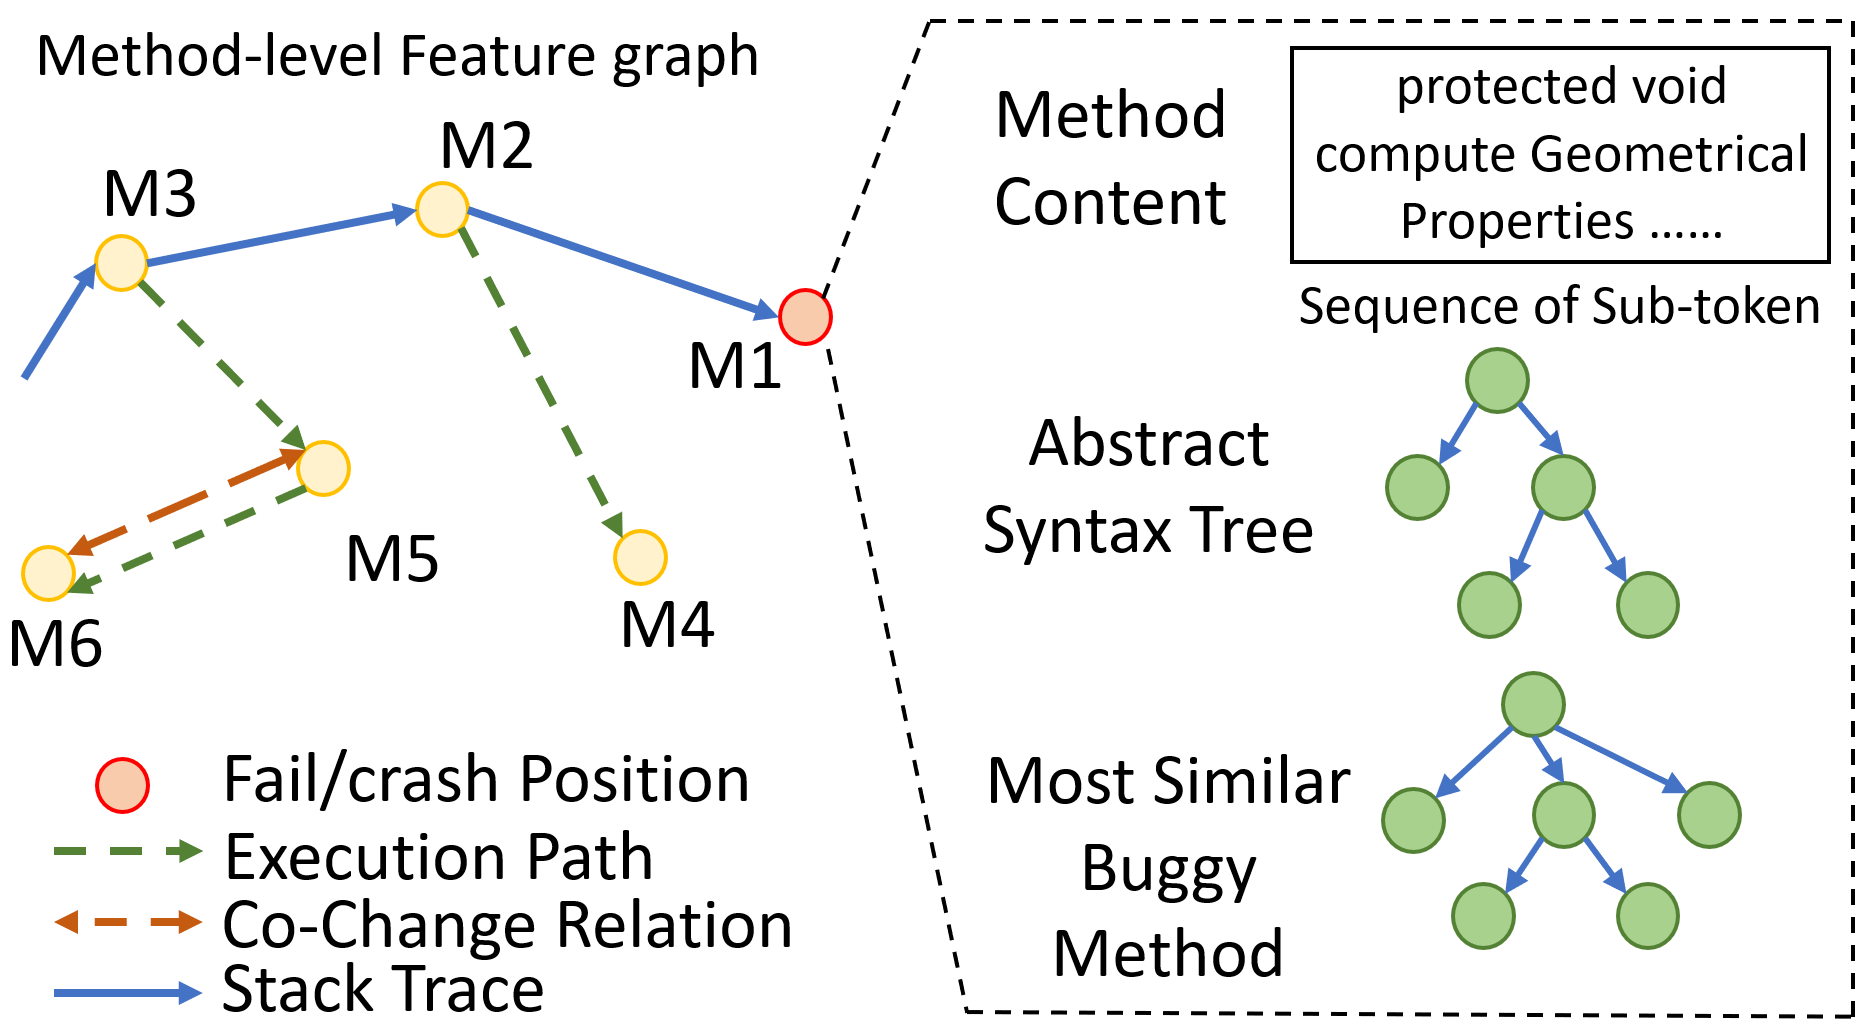
\includegraphics[width=3in]{graphs/step-1-method.png}
        \vspace{-6pt}
        \caption{Method-level Feature Extraction}
	\label{method-level-feature-extraction}
\end{figure}

%For the method level, \tool uses the method as the basic unit. And for each method, \tool extracts three key features, including the method content, abstract syntax tree (AST), and the most similar buggy method. 1> For the method content, \tool collect the source code of each method $M$ and link each statement $S_m$ one by one in $M$ as a sequence $Seq_m$ to represent the method content. \tool removes all special characters and uses CamelCase to break down the tokens in the sequence into sub-tokens to reduce the influence of biases. For example, in the Figure \ref{method-level-feature-extraction}, the method content feature in the method $M1$ shows the extracted sequence of sub-tokens $protected void compute ......$. The source code is listed on the input of the Figure \ref{statement-level-feature-extraction}. 2> As for the AST, \tool generates abstract syntax tree $Tree_m$ for each method $M$ by using JDT package \cite{JDT}. The generated AST looks like the example shown on the abstract syntax tree feature in Figure \ref{method-level-feature-extraction}. 3> When extracting the most similar buggy method feature, \tool breaks down the methods into the sequence of sub-tokens just like the method content feature. It then uses GloVe \cite{pennington2014glove} to learn the embedding for each sub-token and replace the sub-tokens with the embedding vectors. After this, \tool calculates the cosine similarity between the current method $m$ and all other buggy methods in the commit history (before the current bug) to find the most similar buggy method $m_b$. For this buggy method, \tool also uses the JDT package to generate the AST for $m_b$. The most similar buggy method feature in Figure \ref{method-level-feature-extraction} shows a possible example for it.

%For the \underline{relations} among methods, we encode them in the
%method-level feature graph
%(Figure~\ref{method-level-feature-extraction}).

We encode as the edges three types of \underline{relations}:

1) {\em \underline{Calling relation in stack trace}}: we encode into
the feature graph the calling relations in a stack trace of a failed
test case as we ran it.
%
In Figure~\ref{method-level-feature-extraction}, a blue edge connects
$M_i$ to $M_j$ for that relation.
%if $M_i$ calls $M_j$ and they both belong in a stack trace.
Because the stack trace can be very long, from the failing/crash
point, we collect only part of the stack trace with $n$ levels of
depth from that point. Following a prior
work~\cite{crashlocator-issta14}, in our experiment, we set $n$=10.

%After having these three features for each method, \tool uses three kinds of edges to link them as a graph. First of all, \tool runs test cases for the project. If a test case $t_i$ failed, \tool collect the stack trace for the test case $t_i$. Because the stack trace is sometimes too long, using the crashed position as the root, \tool only picks part of the stack trace $st_i$ with the depth of ten in consideration. It means that on the stack trace $st_i$, there are at most ten methods include $m_1, m_2, ..., m_{10}$ where $m_1$ is the crashed position. For every two method $m_j$ and $m_{j+1}$ among these methods, $m_{j+1}$ calls the $m_j$ in the stack trace. The edge $E_m^s$ direction in it is always from $m_{j+1}$ point to $m_j$. For example, in the Figure \ref{method-level-feature-extraction}, the crashed method is $M1$ and the blue solid edges are the stack trace $st_i$. The figure shows that in the stack trace, $M3$ comes out before $M2$ and $M2$ comes out before $M1$.

2) {\em \underline{Calling relations in an execution trace}}:
%we also enhance the feature graph with the calling relations in an
%execution trace.  The calling relations among any two methods that
%are not in the stack trace but in the execution trace, are also added
%to enhance the method-level feature graph. The idea is that the
%calling relations are important to detect faults either they are in
%the stack traces or execution traces.
Similar to the stack trace, an execution trace can be very long from
the failing/crash point. Thus, we keep the methods with only $m$
levels of length in calling relations from that point. In our
experiment, we use
$m$=10. Figure~\ref{method-level-feature-extraction} illustrates a few
calling relations (in green color) in execution traces.

3) {\em \underline{Co-change/co-fixing relation}}: Such a relation
exists between two methods that were changed/fixed in a commit. Such
an edge is made into two one-directional ones (e.g., $M_5
\leftrightarrows M_6$ in
Figure~\ref{method-level-feature-extraction}).

%The second type of edge is the execution path.

%By using each method $m_j$ in the stack trace $st_i$ as the root method, \tool expands the stack trace $st_i$ by adding the executed methods into the graph. The direction of the execution edges $E_m^e$ is also the same as the call direction. Also, because sometimes the execution path may be very long for a method, we only keep the methods $m_k$ within ten steps from the crashed position $m_1$ that means in the graph, from node $m_k$ to $m_1$, the steps are no more than ten (when counting the steps, \tool ignore the edge direction). The green dotted line in Figure \ref{method-level-feature-extraction} shows an example for this type of edge. With the Figure \ref{method-level-feature-extraction}, the green dotted line reflects the relationship that when running the test case $t_i$ on $M2$, it also executes the method $M4$ based on the method call. And then, it executing the $M3$, it executes the method $M5$, and within $M5$, it also executes method $M6$ based on the method calls inside the methods.

%The third type of edge is the co-change relation. For this,  \tool collects all commit history from the input java project. If more than one method has changed in one commit, we mark it as a co-change. The co-change contains all the methods that changed together in this commit. To add the co-change relation as one type of edge, \tool makes the co-change relation become a two-directional edge $E_m^c$ (e.g. The orange edge between $M5->M6$ and $M6->M5$ in the Figure \ref{method-level-feature-extraction}).

%
%\begin{itemize}%
%	\item Graph: 
%	\begin{itemize}
%		\item Stack Trace: \tool runs test cases for the project. If a test case $t_i$ failed, \tool collect the stack trace for the test case $t_i$. Because the stack trace may be very bug, by using the crashed position as the root, \tool pick part of the stack trace $st_i$ with the depth of ten. It means that on the stack trace $st_i$, there are ten methods include $m_1, m_2, ..., m_{10}$ where $m_1$ is the crashed position and for every two method $m_j$ and $m_{j+1}$ among them, $m_{j+1}$ calls the $m_j$ in the stack trace. The edge $E_m^s$ direction in it is always from $m_{j+1}$ point to $m_j$ \tool uses $st_i$ as the base graph and the relationship information in $st_i$ is the dynamic information. 
%		\item Execution Path: As for the failed test case $t_i$, \tool also analyzes the execution path. By using each method $m_j$ in the stack trace $st_i$ as the root method, \tool expands the stack trace $st_i$ by adding the executed methods into the graph. The direction of the execution edges $E_m^e$ is also the same as the call direction. Also, because sometimes the execution path may be very long for a method, we only keep the methods $m_k$ within ten steps from the crashed position $m_1$ that means in the graph, from node $m_k$ to $m_1$, the steps are no more than ten (when counting the steps, \tool ignore the edge direction). The added execution information here is the dynamic edge.
%		\item Co-change Information: \tool collects all commit history of the input java project. If more than one java method has changed in one commit, we mark it as a co-change. The co-change contains all the methods that changed together in this commit. Because the co-change does not have the direction, there is one non-directional edge $E^c$ between every two methods in this co-change to represent the co-change relationship. In order to add the co-change relationship into the stack trace, \tool makes the non-directional edge $E^c$ become a two-directional edge $E_m^c$ (e.g.$method_A -> method_B$ and $method_B -> method_A$). This type of edge is the static edge.
%	\end{itemize}
%	\item Node Features: 
%	\begin{itemize}
%		\item Method Content: \tool collect the source code of each method $M$ and link each statement $S_m$ one by one in $M$ as a sequence $Seq_m$ to represent the method content. \tool removes all special characters and uses CamelCase to break down the tokens in the sequence into sub-tokens to reduce the influence of biases. For example, the $setTagAsStrict$ can be break down into $set, Tag, As,$ and $Strict$. The processed sequence of sub-tokens $Seq^p_m$ is used to represent the method content in \tool. This feature is one of the static features that \tool collects from the source code to represent the method.
%		\item Method Structure: \tool generates abstract syntax tree $Tree_m$ for each method $M$ by using JDT package \cite{JDT}. Each tree $Tree_m$ represent the structure of the relevant method $m$. This is one of the static feature that \tool collect from the source code to represent the method.
		%\item Similar Buggy Method: \tool breaks down the methods into the sequence of sub-tokens just like method content feature and then uses GloVe \cite{pennington2014glove} to learn the embedding for each sub-token and replace the sub-tokens with the embedding vectors. After this, \tool calculate the cosine similarity between the current method $m$ and all other buggy methods in the commit history (before current bug) to find the most similar buggy method $m_b$. This is one of the static feature that \tool collect from the source code to represent the method.
%	\end{itemize}	
%\end{itemize} 

\begin{figure}[t]
	\centering
	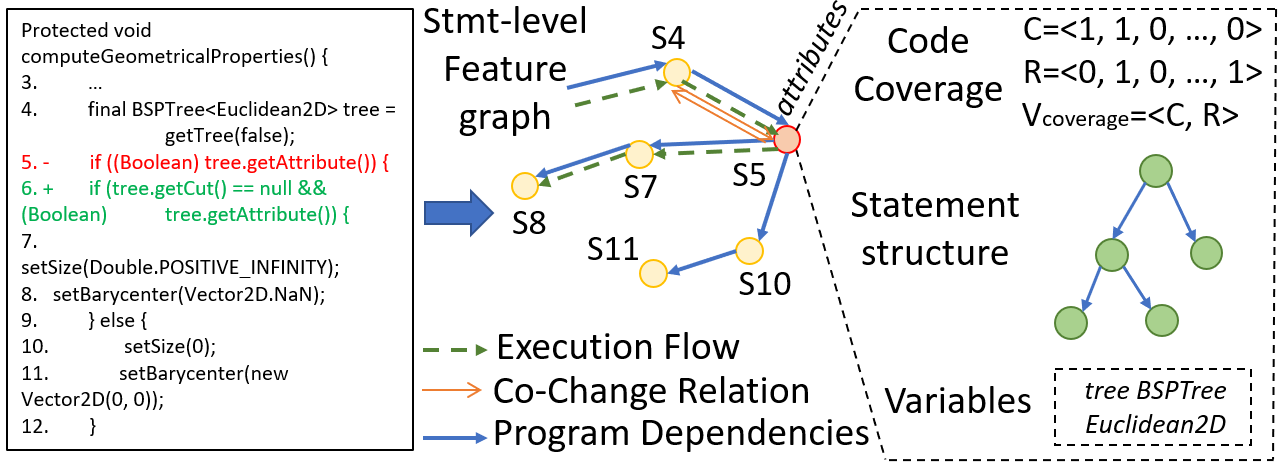
\includegraphics[width=3.6in]{graphs/step-1-statement-2.png}
        \vspace{-19pt}
	\caption{Statement-level Feature Extraction}
        \vspace{-5pt}
	\label{statement-level-feature-extraction}
\end{figure}


\subsection{Statement-level Feature Extraction}

For each statement, we extract the following \underline{attributes}.

1) {\em \underline{Code coverage}}: we run the test cases and collect
code coverage information. For each statement $s$, we use a vector $C
= <c_1, c_2, ..., c_K>$ ($K$ is the number of test cases) to encode
code coverage in which $c_i=1$ if the test $t_i$ covers $s$, and
$c_i=0$ otherwise. We use another vector $R = <r_1, r_2, ..., r_K>$ to
encode the passing/failing of a test case in which $r_i=1$ if the test
case $t_i$ is a passing one and $r_i=0$ otherwise. $R$ is common for
all the statements. We concatenate $C$ and $R$ for each statement to
obtain the code coverage feature vector $V_{Cov} = <c_1, c_2, ...,
c_K, r_1, r_2, ..., r_K>$.
%
We used DeepRL4FL's test ordering algorithm~\cite{icse21-fl} as
ordering of test cases is useful for FL.
%
For the different numbers of test cases across files, we perform zero
padding to make the vectors have the same length.

2) {\em \underline{AST structure}}: we extract the sub-tree in the AST that
corresponds to the current statement.

3) {\em \underline{List of variables}}:
%because the variables in a method are important in FL, we also collect
%the list of variables and their types into a sequence.
We break the names into sub-tokens. In
Figure~\ref{statement-level-feature-extraction}, the sequence for the
variable list is [\code{tree}, \code{BSPTree}, \code{Euclidean2D},...].




%For the statement level,  \tool uses the statement as the basic unit. And for each statement, \tool extracts three key features, including the code coverage information, sub-AST, and variables to represent the statement. 1> As for the code coverage information, \tool runs the relevant test cases for the input project. For the test case $t_i$, if it passes the statement $s_i$, \tool uses $c_i = 1$ to represent it while if it does not pass the statement $s_i$, \tool uses $c_i = 0$ to represent it. By linking all $c_i$ together, \tool can get $C = <c_1, c_2, ..., c_i>$. Also, \tool uses $r_i = 1$ to represent the the condition $passed$ and uses $r_i = 0$ to represent the condition $failed$ for the test case $t_i$ . By linking all $r_i$ together, \tool can get $R = <r_1, r_2, ..., r_i>$. By concatenate $C$ and $R$, \tool extract the code coverage information feature by $V_{coverage} = <c_1, c_2, ..., c_i, r_1, r_2, ..., r_i>$. The code coverage information feature in Figure \ref{statement-level-feature-extraction} shows an example of it.

%2> For the sub-AST, it is very similar to the method level. By using JDT package, \tool can extract the AST for the whole method. And then, \tool searches for the nodes that appears in the statement. By collecting all these nodes and the edges between then, \tool can extract the sub-AST for the statement.

%3> For the variables feature, for each statement, \tool collects all the variables $V$ that appeared in it and for each variable $v$ in $V$, \tool uses the $(variable_name variable_type)$ to represent it. Then \tool links all variables $V$ together with $,$ as a sequence $Seq_s$ as one of the static feature that \tool collect from the source code to represent the statement. For example, in Figure \ref{statement-level-feature-extraction}, \tool goes through the statement at $line 5$ in the input method and finds that only one variable $tree$ appears in the statement at $line 5$. So the variable feature here should be like $variable_name variable_type$ where $variable_name$ is $tree$ and $variable_type$ is $BSPTree Euclidean2D$.

%Tien
We encode the following types of \underline{relations} among
statements:

1) {\em \underline{Program dependence graph (PDG)}}: as suggested
in~\cite{icse21-fl}, the relations among statements in an PDG are
important in FL, thus, we integrate them into the feature graph. In
Figure~\ref{statement-level-feature-extraction}, the blue edges
represent the relations in the PDG for the given code.  The statement
at line 4 has a control/data dependency with the one at line 5, which
connects to the ones at lines 7--8, and to the ones at lines 10--11.

2) {\em \underline{Execution flow in an execution trace}}: if two
statements are executed consecutively in an execution trace, we will
connect them together. In
Figure~\ref{statement-level-feature-extraction}, we have the execution
flow $S_5 \rightarrow S_7$, $S_7 \rightarrow S_8$.

%With these three features, similar to the method-level, \tool builds three types of edges to link the statements together as a graph. The first type of edge is the program dependency edge (PD). \tool builds the PD by using the tool soot \cite{soot} for the method $m$. For example, in Figure \ref{statement-level-feature-extraction}, the blue edges are the PD edges and they show that in method $m$, statement at $line 4$ controls the statement at $line 5$. And statement at $line 5$ can control the statements at $line 7-8$ and the statements at $line 10-11$.

%The second type of edge that \tool extracts is the execution flow $E_s^e$. The execution flow is the order that the failed test case $t_i$ went through in the method $m$. For example, the green dotted edges are the execution flow. Within it, we can see that the test case executes $S7-S8$ but did not go through $S10-S11$. Even though in the PD, $S5$ is linked by $S10-S11$. It means that when running the test case $t_i$, it will not pass the $S10$ and $S11$ because of the if checking in $S5$.

3) {\em \underline{Co-change/co-fixing relation}}: we maintain the
co-change/co-fixing relations among statements. In
Figure~\ref{statement-level-feature-extraction}, $S_4$ and
$S_5$ have been changed in a commit, thus, two co-change
edges connect them.

%The last type of edge $E_s^c$ is the co-change relation in the statement level. \tool collects the co-change information for the commit about the statements that changed together before in the current method $m$ and one commit. In Figure \ref{statement-level-feature-extraction}, the commit history shows that $S4$ and $S5$ used to be changed together before. Hence, there is an orange edge that represents the co-change relation between $S4$ and $S5$.


%\begin{itemize}
%	\item Graph: 
%	\begin{itemize}
	%	\item Program Dependency Graph (PDG): \tool builds the PDG by using the tool soot \cite{soot} for the method $m$ that contains the statements that \tool want to analyze. \tool uses the generated PDG as the base graph. Within this graph, there are two types of edges including data dependency and control dependency. Both of these two types of edges are the static edges.
	%	\item Execution Path: \tool collects the execution path of the failed test case $t_i$ within the method $m$ and adds them into the PDG by adding a new type of edge $E_s^e$. The new edge direction is the same as the execution order. This type of edge is the dynamic edge.
%		\item Co-change Information: Similar to the method-level, \tool collects the co-change information for the commit about the statements that changed together before in one commit and the current method $m$. As for adding the co-change information into the PDG, \tool also creates the two-directional edge $E_s^c$ similar to the method level. This type of edge is the static edge.
%	\end{itemize}
%	\item Node Features: 
%	\begin{itemize}
	%	\item Code Coverage Information: \tool runs the relevant test cases for the input java project. For the test case $t_i$, if it passes the statement $s_i$, \tool uses $c_i = 1$ to represent it while if it does not pass the statement $s_i$, \tool uses $c_i = 0$ to represent it. By linking all $c_i$ together as $C = <c_1, c_2, ..., c_i>$, $C$ is considered by \tool as one of the dynamic feature.
	%	\item Statement Structure: Similar to the method-level, \tool generates a sub abstract syntax tree $Tree_s$ for each statement $S$ by using JDT \cite{} package. Each tree $Tree_s$ represent the structure of the relevant statement $s$. This feature is one of the static features that \tool collects from the source code to represent the statement.
	%	\item Variables: For each statement, \tool collects all the variables $V$ that appeared in it and for each variable $v$ in $V$, \tool uses the $(variable_name variable_type)$ to represent it. Then \tool links all variables $V$ together with $,$ as a sequence $Seq_s$ as one of the static feature that \tool collect from the source code to represent the statement. For example, the variables in the statement in line 3 in Figure \ref{fig:motiv} include $root$ and $sourceMap$. \tool generates the feature for them as $root Node, sourceMap SourceMap$ where $root$ and $sourceMap$ are the names and $Node$ and $SourceMap$ are the types.
%	\end{itemize}	
%\end{itemize} 
